% Preamble
\documentclass[12pt, a4paper, twoside]{article}
\usepackage[a4paper, left=0.75in, right=0.75in, top=1in, bottom=1in]{geometry}
\usepackage{lipsum, verbatim, fancyhdr, lastpage, graphicx, hyperref, amsmath} % indentfirst 
\usepackage[backend=bibtex]{biblatex}
\graphicspath{{./plots/}}
\addbibresource{ref.bib}
% Top Matter
\hypersetup{
	colorlinks   = true,
	urlcolor     = blue, 
	linkcolor    = blue, 
	citecolor   = red
}
\pagestyle{fancy}
\fancyhead[CO, CE]{CS 725: Foundations of Machine Learning (Autumn 2023) --- Project}
\fancyhead[LO, LE, RO, RE]{}
\fancyfoot[CO, CE]{Page \thepage\ of \pageref{LastPage}}
\fancyfoot[LO, LE, RO, RE]{}
% \bibliographystyle{plain}

\title{\vspace{-0.5in}\textbf{CS 725: Foundations of Machine Learning \\
Midterm Project Report}}
\author{CV Mavericks\footnote{The project has undergone revisions based on the feedback provided on 18/10/2023. Initially, the project focused on \emph{Image-Based Disease Diagnosis using Deep Learning}. The new project concept has received approval from Krishnakant Bhatt (21q050016@iitb.ac.in).}\\
23m2154, 23m2156, 23m2157, 23m2158, 23m2162}
\date{October 31, 2023}

% Main Matter
\begin{document}
\maketitle
\thispagestyle{fancy}

\begin{abstract}
Our project addresses the limitations of current food image datasets in accurately estimating calories. We introduce a food image dataset that includes both food annotations and detailed volume and mass records for each item, along with a calibration reference. Our dataset comprises 2978 images, each accompanied by annotations and essential food metrics. To estimate the calorie content of food in this dataset, we employ a deep learning approach utilizing Faster RCNN for food detection and a GrabCut algorithm to outline the contours of each food item. With this information, we calculate the volume and subsequently, the calorie content of each food.
\end{abstract}

\section{Problem Statement}
Estimating the calorie content from food images requires the food image datasets which faces a critical challenge in accurately estimating calorie content due to the choice of object detection algorithm and volume estimation method. This project aims to fill this gap by using a detailed food image dataset provided by ECUST\cite{liang}. It includes precise food annotations, along with volume, mass records, and a reliable calibration reference (one Yuan coin) for each item. This dataset is a collection of 2978 images, each meticulously annotated and supplemented with necessary food metrics i.e. volume, density, calorie content etc. To achieve accurate calorie estimation, a deep learning methodology is employed. This involves the adaptation of faster Region-based Convolutional Neural Networks (RCNN) for precise food detection, followed by the implementation of the GrabCut algorithm to precisely outline the contours of each food item. The segmented images would be utilized to calculate the volume and, subsequently, the calorie content of each food item.
\par
The project aims to address two key challenges in dietary assessment from food images:
\begin{description}
	\item[Detection and Classification of Food Items:] Accurate identification and categorization of food items from images represent the initial hurdle. Existing methodologies often fall short in providing precise detection and classification. This project seeks to leverage advanced techniques, particularly faster RCNN, to enhance the capability to not only detect but also classify food items within images. By employing faster RCNN, the system aims to achieve an improvement in the accuracy and efficiency of food item recognition.
	
	\item[Estimation of Food Volume for Calorie Content Determination:] 
	The second significant challenge lies in estimating the volume of identified food items, a crucial step in determining their calorie content. Traditional approaches struggle to provide the necessary precision for this task. To overcome this limitation, the project proposes the integration of GrabCut, an advanced segmentation algorithm. By applying GrabCut, the system aims to accurately delineate the contours of each food item, enabling precise volume estimation. This, in turn, facilitates a more accurate and reliable assessment of calorie content.
\end{description}
\par
By combining the faster RCNN for food item detection and classification with GrabCut for precise volume estimation, this project seeks to accurately estimate the calorie content from food images. The successful execution of this approach promises to benefit individuals seeking improved dietary choices, weight management, fitness goals, and specific dietary requirements.

\section{Proposed Solution Approach}
The solution methodology for estimating the calorie content from food images can be summarized as follows:
\begin{description}
	\item[Object Detection:] Our aim is to help people who want to keep track of the calories they consume. We would create a system that works with a smartphone. Before eating, users need to take pictures of their food from the top and side views. They should include a One Yuan coin in each picture. For the top view, we use faster RCNN to recognize the types of food and draw an outline or bounding box around them in the photos. We do the same for the side view. The primary goal of the faster RCNN is to develop a unified architecture that not only detects objects within an image but also locates the objects precisely in the image. It combines the benefits of deep learning, CNN, and region proposal networks(RPN) into a cohesive network, which significantly improves the speed and accuracy of the model. When we give it a picture, it gives us boxes around the objects. It also tells us what type of object it thinks it is.
	
	\item[Image Segmentation:] Before figuring out the volume, we first break down each box into its separate parts. We would use something called GrabCut algorithm. It's a way to process images that helps us focus on specific areas. Normally, users would have to highlight areas themselves, but we've made it so the system can do this on its own. After this step, we get a precise outline or contour of each food item. Then, we can estimate the volume and calorie content. This process uses an image processing approach to segment each bounding box. As mentioned above, the bounding boxes around the object that GrabCut needs can be provided by faster RCNN. After segmentation, we can get a series of food images stored in matrix, but with the the values of the background pixels being replaced by zeros. This will leave only the foreground pixels.
	
	\item[Calorie Estimation:] The user needs to provide the image clicked from both side and top view along with the One Yuan coin. According to the One Yuan coin detected in the top view, the true size of a pixel is known. Similarly, we know actual size of of a pixel in the side view. Then we use different formulas to estimate volume of each food. After getting volume, food’s calorie is obtained by searching related calorie tables. 
\end{description}

\section{Code Survey}
\subsection{Object Detection in Faster RCNN}
\subsubsection{PyTorch}
We have explored the official PyTorch documentation for using Faster RCNN model by importing from torch-vision and reference code to understand the use of functions implemented and the arguments to be passed. The GitHub link consists of source code of implementation of Faster RCNN in PyTorch used in documentation. The Medium article is walk-through of implementing Faster RCNN from scratch in PyTorch. The article implements the RPN network for creating anchor boxes and uses VGG16 as the backbone architecture. The PyTorch tutorial helps in understanding how to fine tune Pre-trained object detection models for custom dataset. The link fine tunes a mask RCNN model and explains how to change the underlying backbone architecture.
\begin{enumerate}
	\item \href{https://pytorch.org/vision/main/models/faster_rcnn.html}{Faster RCNN in PyTorch}
	\item \href{https://github.com/pytorch/vision/blob/main/torchvision/models/detection/faster_rcnn.py}{Source code of Faster RCNN in PyTorch}
	\item \href{https://medium.com/@fractal.ai/guide-to-build-faster-rcnn-in-pytorch-42d47cb0ecd3}{Faster RCNN from scratch}
	\item \href{https://pytorch.org/tutorials/intermediate/torchvision_tutorial.html}{Fine tuning pre-trained RCNN model}
\end{enumerate}

\subsubsection{TensorFlow}
We have gone through the TensorFlow documentation on object detection API and explanation on different object detection models --- one of them being Faster RCNN. The GitHub link consists of source code of Faster RCNN implemented by TensorFlow on different backbone architectures.
\begin{enumerate}
	\item \href{https://www.tensorflow.org/hub/tutorials/object_detection}{Faster RCNN in TensorFlow}
	\item \href{https://github.com/tensorflow/models/blob/master/research/object_detection/models/faster_rcnn_pnas_feature_extractor_tf1_test.py
	}{Source code of Faster RCNN in TensorFlow}
\end{enumerate}

\subsection{GrabCut Algorithm for Extracting Foreground from Bounding Boxes}
The \href{https://docs.opencv.org/3.4/d8/d83/tutorial_py_grabcut.html}{OpenCV documentation} for understanding the GrabCut algorithm for foreground extraction and sample code for understanding its implementation. 

\subsection{Different Backbone Architectures Used for Implementing Faster RCNN}
Different backbone architectures can be used for implementing Faster RCNN. Below are the links to the architectures we will be going through and their source code implementation in Keras. The study of different backbone architectures will help select the right model for our problem statement.
\begin{enumerate}
	\item \href{https://keras.io/api/applications/resnet/}{Resnet50} 
	\item \href{https://keras.io/api/applications/vgg/}{VGG16}
	\item \href{https://keras.io/api/applications/mobilenet/}{MobileNet}
	\item \href{https://keras.io/api/applications/inceptionresnetv2/}{InceptionResnetV2}
\end{enumerate}

\subsection{Region Proposal Network Implementation}
The key feature of implementing Faster RCNN is its Region Proposal Network (RPN). The \href{https://martian1231-py.medium.com/region-proposal-network-rpn-in-faster-rcnn-from-scratch-in-keras-1311c67c13cf}{article} gives a detailed walk-through of implementing the RPN network while covering the important aspects of its implementation which will help us understand the network and allow us the ability to make changes as per our need.

\section{Datasets}
We utilize the ECUST dataset, which encompasses 19 diverse food types including apple, banana, bread, bun, doughnut, egg, fired doughnut, grape, lemon, litchi, mango, mooncake, orange, peach, pear, plum, kiwi, sachima, and tomato as shown in Figure \ref{F:table}. The model is trained on a total of 2978 images from this dataset. Each food item is captured in multiple sets of photos, showcasing both its top and side views (see Figure \ref{F:sample}). Each image is calibrated using a one Yuan coin as shown in Figure \ref{F:coin}, and no more than two food items are present in a single picture. Additionally, all images in the dataset are smaller than 1000 by 1000 pixels. The dataset provides density and energy content information for all 19 food items.
\par
To ensure accurate measurement of food volume and mass, foods that are sufficiently large, stable, and less likely to deform. are selected. Foods with small volumes, like peanuts, are challenging to measure accurately and can lead to significant errors when compared to their actual volume. In ECUST dataset, every food item is presented in its entirety. In the dataset, the whole foods, such as entire apples rather than sliced ones were prioritized to facilitate volume and weight measurements. Photos were taken in various mobile devices, under lighting conditions, including low light settings. Different shooting angles were used for top and side views. The position of the food in images was flexible, as long as it was fully captured. A One Yuan coin was chosen as the calibration object due to its common availability, with a diameter of 25.0mm.

\begin{figure}[p]
	\centering
	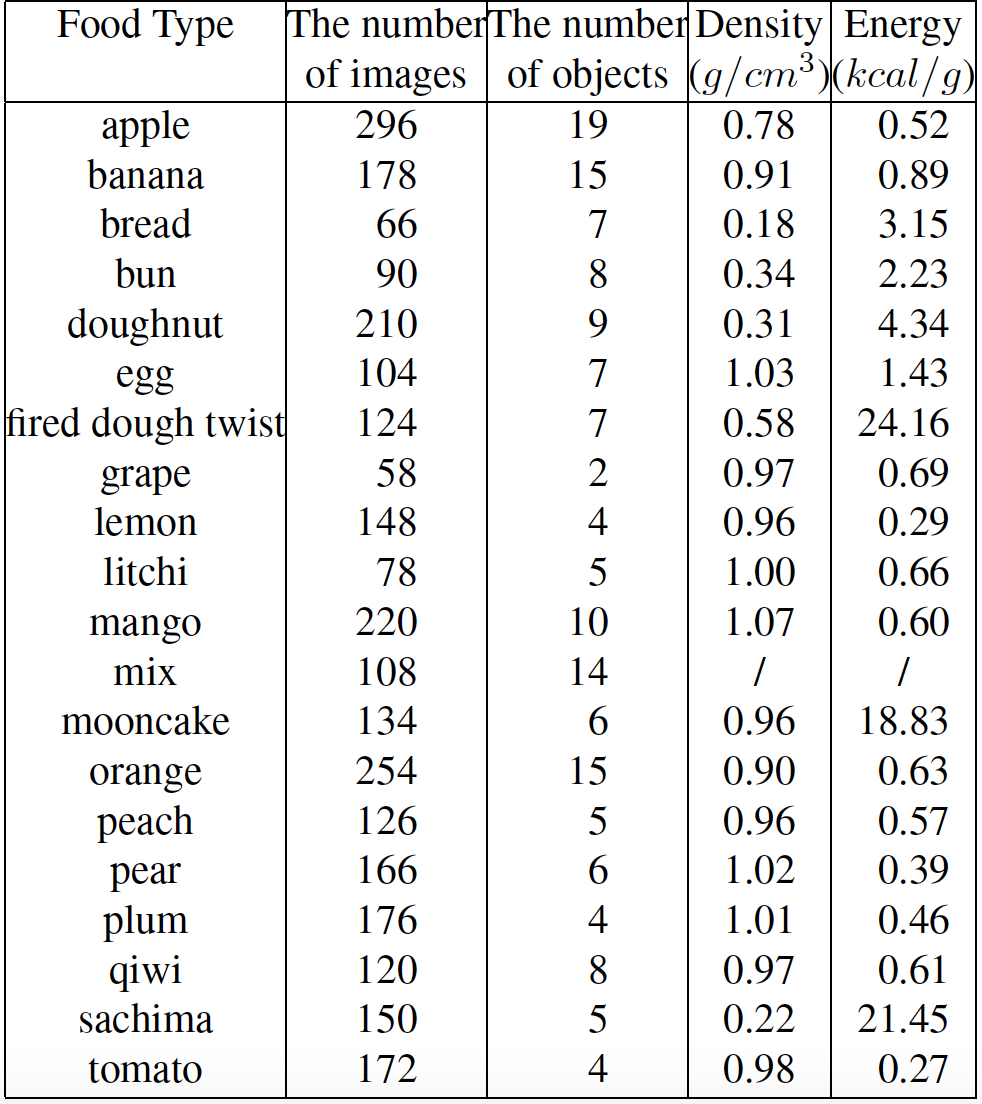
\includegraphics[width=\textwidth]{table}
	\caption{Details of food item from ECUST dataset}
	\label{F:table}
\end{figure}
\begin{figure}[p]
	\centering
	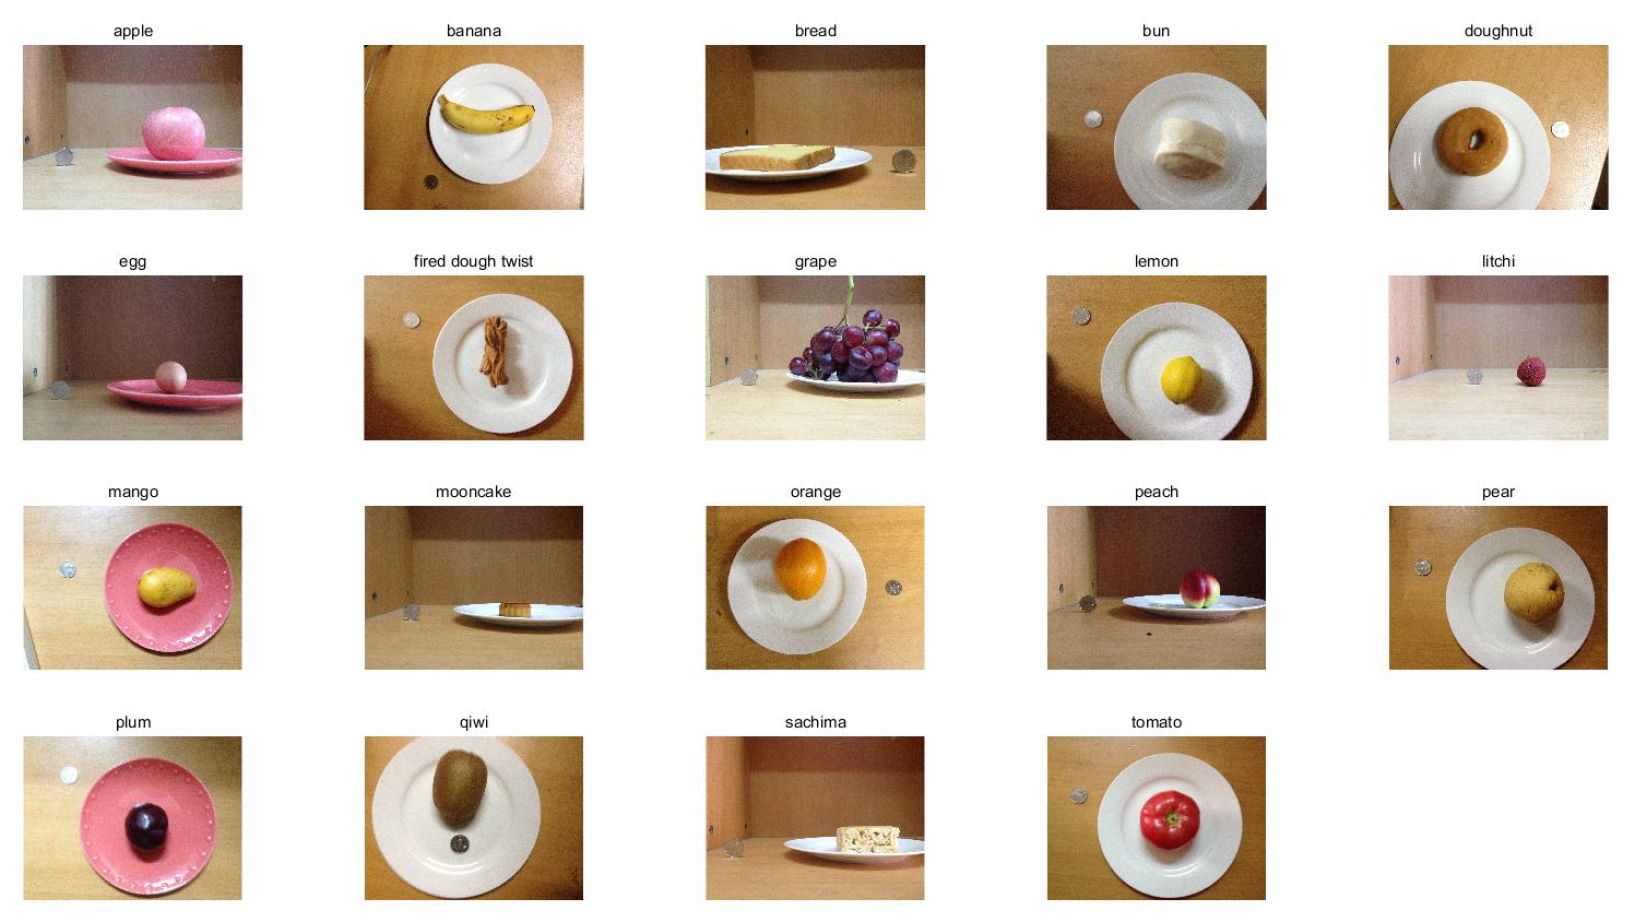
\includegraphics[width=\textwidth]{sample}
	\caption{Sample food items from ECUST dataset}
	\label{F:sample}
\end{figure}
\begin{figure}[p]
	\centering
	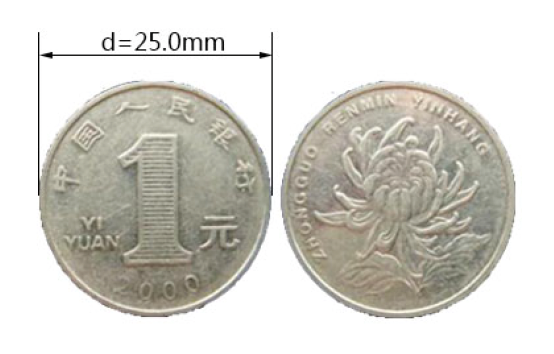
\includegraphics[width=0.75\textwidth]{coin}
	\caption{Dimension of One Yuan coin}
	\label{F:coin}
\end{figure}

\section{Implementation Details}
\subsection{Faster RCNN}
This algorithm\cite{rcnn} takes an image as input and produces a convolution feature map. It utilizes a separate network to suggest potential regions of interest. These suggested regions are then reshaped using a Region of Interest (ROI) pooling layer. Offset values for bounding boxes are predicted based on this reshaping, and the images within the proposed regions are classified. Faster RCNN is chosen for image detection due to its superior speed compared to other algorithms like RCNN and Fast RCNN. Anchors play a crucial role in Faster RCNN. An anchor is essentially a box, and in the default setup of Faster RCNN, an image is divided into 9 anchors. Using a well-chosen set of anchors can enhance both speed and accuracy. The Region Proposal Network (RPN) produces a set of boxes or proposals, which are then examined by the classifier and regressor to identify objects.

\subsection{GrabCut Algorithm}
The GrabCut algorithm\cite{grabcut} employs Image Segmentation. In this method, we use a box to define the object, effectively separating it from the background. The outer region of the box represents the background, while the inner portion combines some background and the object. Subsequently, an iterative process designates each pixel as either background or foreground. Initially, the computer makes an educated guess based on user-provided data. Then, we utilize a Gaussian mixture model to characterize both the foreground and background. Next, we label pixels as probable foreground or probable background, designating others as unknown.
\par
In this algorithm, every pixel becomes a node in a graph. Additional nodes like source and sink nodes are introduced. The source node connects to the foreground pixels, while the sink node connects to the background pixels. The likelihood of a pixel being foreground or background influences the edge weights connecting the pixels to these nodes. The similarity between pixels, indicated by the edge information, determines these weights. If there's a substantial color difference between pixels, a low weight is assigned to the edge. Following this, the graph undergoes Segmentation using min-cut. This operation divides the graph into two parts, separating the source and sink nodes, and does so with the least possible cost. The total weights of the cut edges constitute the cost function. Post-cut, all pixels connected to the Source node become foreground, while those linked to the Sink node become background. This process continues until the classification stabilizes.

\subsection{Volume Calculation}
To estimate the volume\cite{vol}, we calculate the scale factors based on calibration objects. We use a One Yuan coin to show the specific process of calculating the volume. The diameter of the coin is 2.5 cm, and the side view’s and top view's scale factor ($\alpha_S$ and $\alpha_T$) is calculated with Equation \ref{E:as} and \ref{E:at}.
\begin{align}
	\alpha_S &= \frac{2.5}{(W_S + H_S)/2} \label{E:as}\\
	\alpha_T &= \frac{2.5}{(W_T + H_T)/2 \label{E:at}}
\end{align}
\par
Where $W_S$ and $H_S$ are the width and height of bounding box in side view. Moreover, $W_T$ and $H_T$ are the width and height of bounding box in top view.
\par
Furthermore, we divide the foods into three categories based on shape: ellipsoid, column, irregular. Different volume estimation formula will be selected for different types of food, according to Equation \ref{E:vol}. 
\begin{equation}\label{E:vol}
	v = 
	\begin{cases}
		\beta \cdot \frac{\pi}{4} \cdot \alpha_S^3 \cdot \sum_{k=1}^{H_S} (L^k_S)^2, &\text{if shape is ellipsoid} \\
		\beta \cdot  s_T \cdot \alpha_T^2 \cdot H_S \cdot \alpha_S, &\text{if shape is column} \\
		\beta \cdot  s_T \cdot \alpha_T^2 \cdot \alpha_S \cdot \sum_{k=1}^{H_S} \left(\frac{L^k_S}{L_S^{max}}\right)^2, &\text{if shape is irregular} 
	\end{cases}
\end{equation}
\par
Where $L^k_S$ is the number of foreground pixels in side view of row $k$ ($k \in 1, 2, 3, \dots , H_S$). $L^{max}_S = \max_{k} L^k$, it records the maximum number of foreground pixels in side view. $\beta$ is a compensation factor (default value = 1.0).  $s_T$ is the surface area of the top view.
\par
After estimating the volume, the next step is to estimate each food’s mass ($m$ in $g$). It can be calculated in Equation \ref{E:mass}, Where $v$ represents the volume of food in $cm^3$, and  $\rho$ represents its density value in $g/cm^3$. Then the calorie ($C$ in $cal$) of the food can be calculated by Equation \ref{E:cal} using the unit energy ($c$ in $cal/g$).
\begin{align}
	m &= \rho \cdot v \label{E:mass} \\
	C &= c \cdot m \label{E:cal}
\end{align}
\par
The density, unit energy values and shape for each food items can be obtained from ECUST dataset.

\section{Roadmap}
This project aims to estimate the calorie from the food image dataset. The flowchart for implementing the project is shown in Figure \ref{F:roadmap}. The detailed roadmap to implement the project is shown below.
\begin{description}
	\item[Acquiring the ECUST Dataset] Familiarize yourself with the problem statement and the challenges addressed in the project.
	\item[Data Preprocessing] Load and preprocess the dataset. This may include resizing images, normalizing pixel values, and organizing annotations. Explore the dataset to understand its characteristics, such as image dimensions, class distributions, and other relevant statistics.
	\item[Object Detection with Faster RCNN:] Implement the Faster Region-based Convolutional Neural Network (RCNN) for food detection and classification. Train the model on the annotated food images from the ECUST dataset.
	\item[Volume Estimation with GrabCut:] Apply the GrabCut algorithm to segment the food items and accurately delineate their contours. Use the segmented images to estimate the volume of each food item.
	\item[Calorie Content Estimation:] Utilize the obtained volume information, along with density values, to estimate the calorie content of each food item.
	\item[Validation and Evaluation:] Evaluate the performance of the model using appropriate metrics. This may include accuracy, precision, recall, etc.
	\item[Documentation and Reporting:] Document your methodology, code, and results thoroughly. Provide explanations for design choices and algorithm implementations.
\end{description}
\begin{figure}[p]
	\centering
	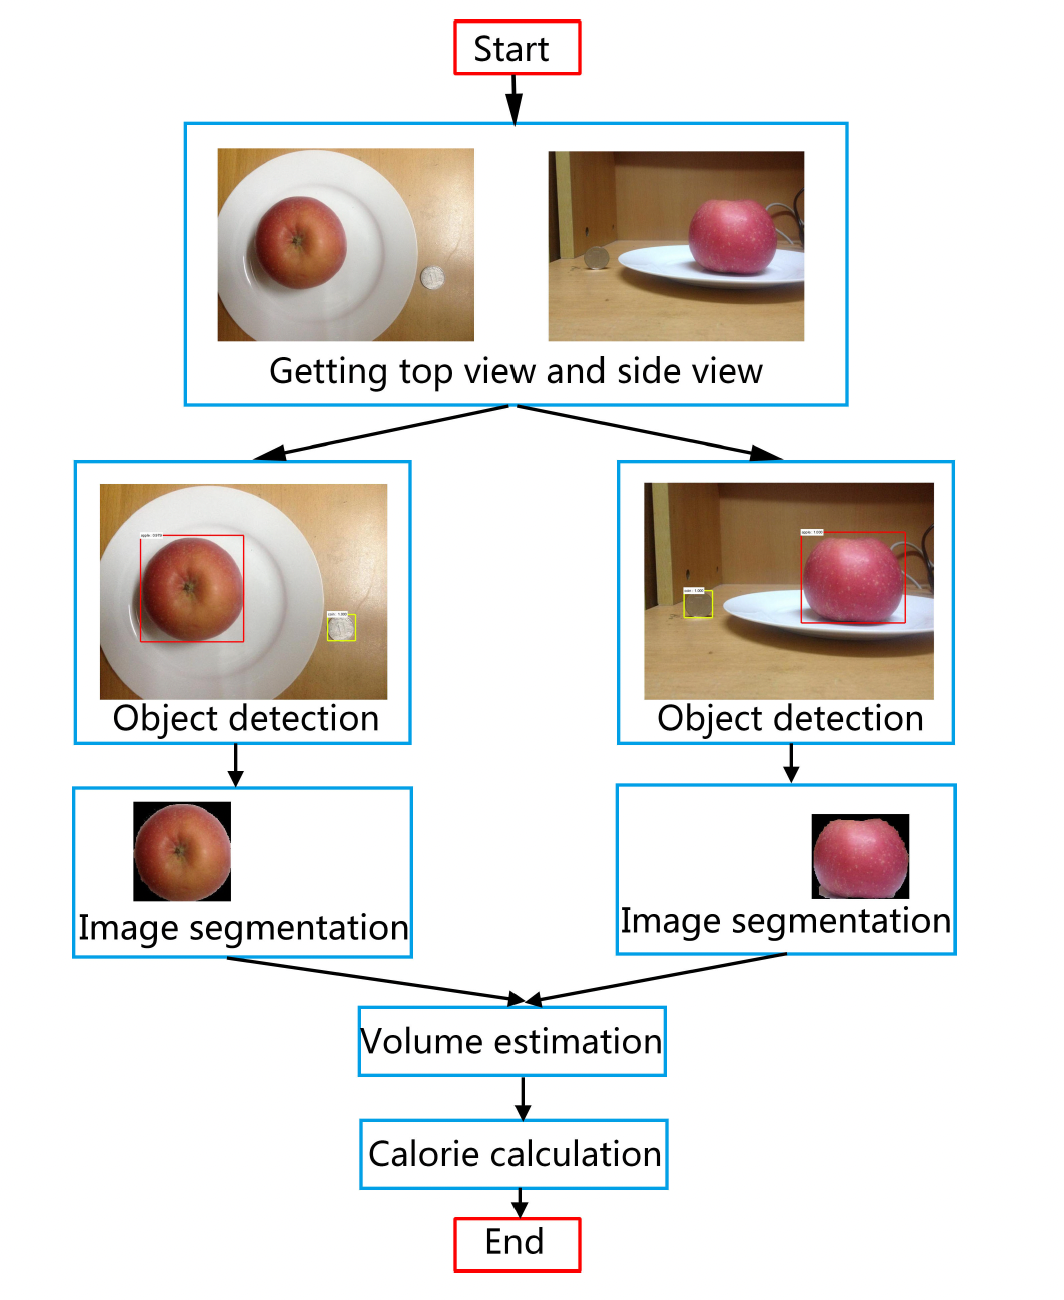
\includegraphics[width=\textwidth]{roadmap}
	\caption{Flowchart to implement the project\cite{liang}}
	\label{F:roadmap}
\end{figure}

\printbibliography
\end{document}